\documentclass{article}

\usepackage{amsmath}
\usepackage{amsthm}
\usepackage{amssymb}
\usepackage{color}
\usepackage{tikz}
\usetikzlibrary{shapes,arrows.meta,backgrounds}
\usepackage{etoolbox}
\usepackage{url} % for urls in bibliography
\usepackage[parfill]{parskip} % no paragraph indents, leave blank line
\usepackage{graphicx}
\usepackage{subcaption}
\usepackage{listings}

\graphicspath{ {./drawio/} }

% Need this to keep the space before theorems when using parfill parskip
% https://tex.stackexchange.com/questions/25346/wrong-spacing-before-theorem-environment-amsthm
\begingroup
    \makeatletter
    \@for\theoremstyle:=definition,remark,plain\do{%
        \expandafter\g@addto@macro\csname th@\theoremstyle\endcsname{%
            \addtolength\thm@preskip\parskip
            }%
        }
\endgroup

\DeclareRobustCommand{\rchi}{{\mathpalette\irchi\relax}}
\newcommand{\irchi}[2]{\raisebox{\depth}{$#1\chi$}} % inner command, used by \rchi

\title{Nitro Protocol}
\author{Tom Close}

\usepackage{mathtools}
\usepackage{bm}
\usepackage{stmaryrd} % for llbracket and rrbracket

\theoremstyle{definition}
\newtheorem{example}{Example}[section]
\newtheorem{defn}{Definition}[section]

\newcommand{\adj}[1]{\llbracket #1 \rrbracket} 
\newcommand{\enf}[1]{[#1]} 

\begin{document}

\maketitle

\section{Motivation}

A blockchain is a device that enables a group of adversarial parties to come to consensus over the contents of a shared ledger, without appealing to a trusted central authority. 
Whether using a proof-of-work or a proof-of-stake algorithm, this process has a cost both in terms of time and in terms of money.
For the Ethereum blockchain, this cost results in an effective limit of around 15 transactions per second being processed on the network.
When compared with the visa network, which can process on the order of 50,000 transactions per second, this limit supports the view that blockchains, in their current form, do not scale.

State channels offer a solution to the blockchain scaling problem.
A state channel can be thought of as a set of updatable agreements between a fixed set of participants determining how a given set of assets should be split between them.
The agreements are updated off-chain through the exchange of cryptographically signed messages between the participants according to some set of previously-agreed update rules. 
The assets in question are held in escrow on the blockchain, in such a way
that they can only be released according to the latest agreement from the state channel.
If the off-chain cooperative behaviour breaks down, for example if one party refuses to sign updates either by choice or due to unavailability, any of the parties can reclaim their share of the assets by presenting the latest agreement to the chain.
An exit game is required to give other parties the opportunity to present a later state, but all parties have the guarantee that they can reclaim their share of the funds within some finite time.

In addition to the increased throughput, state channels bring instant finality to transactions: the moment a channel update is received the participant knows that the assets transferred are now assigned to them.
They cannot access the assets immediately but they have the power to prevent any other party claiming those assets in the future.
The only requirement is that participants need to be live enough to engage in the exit game if an opponent attempts to exit an earlier state.
In practice, the requirement here is to check the chain periodically - at time intervals that are less than, but on the same order of magnitude as, the challenge duration in the exit game.

As the channel updates are created and exchanged off-chain, the channel-update throughput is limited only by the speed of constructing, signing and broadcasting the update.
Given that channel updates only needed to be communicated between participants and the system is therefore highly parallelizable, it is difficult to put a bound on the total transaction throughput of a system of state channels.
In practice the system is only limited by the on-chain operations required to move assets when opening and closing channels.

In this paper, we allow channels to be opened and closed off-chain. We enable the construction of efficient state channel networks.[TODO]

\section{Existing work}

Lightning and raiden
- payment channel networks
- directional

Celer
- directional but with multiple paths
- general conditions

Perun
- virtual payment channels (different from HTLCs)
- but using a validity time
- and then state channel networks
- constrained
[Connext - have removed the time limit with a trade-off of trusting the hub - TODO: check this]

Counterfactual
- thinks about counterfactual instantiation
- also app instance on top, which we collaborated on
- possible to do meta-channels, but the details are not given in the paper and are still being finalized

ForceMove

Our contribution:
- like perun without the time limit
Unconstrained subchannels

\section{State Channel Background}

In this paper, we are focus on the construction of networks of state channels, which we treat separately from the operation of those channels.
For the purpose of this work, we view a state channel and its states purely as a device for enabling a given party to realize a given outcome on-chain, in a sense that we will make precise.
In particular, we do not specify the state format, the update rules, the mechanics of on-chain challenges or how to respond to them.

The ForceMove framework is an example of a state channel framework that specifies all these details. 
The state channel networks presented here were designed to work with ForceMove and we will frequently present examples involving ForceMove channels.
That said, the techniques provided here should be applicable to any state channel framework sharing the features presented in this section.

We start the section by reviewing the properties of ForceMove that are important for Turbo and Nitro \footnote{We give a more complete recap of ForceMove in the appendix.}. 
We then introduce some concepts that will be useful later when reasoning about the correctness of our state channel networks. 

\subsection{ForceMove Channels}

A ForceMove state channel belongs to a set of \textbf{participants}, each defined by a unique cryptographic address.
The private keys corresponding to these addresses are used to sign updates to the channel.
We assume that the signature scheme is unforgeable, so that only the owner of the address has the capability to sign states as that participant.

Each channel has a \textbf{channel address} which is formed by taking the hash of the participant addresses along with a nonce, $k$, that is chosen by the participants in order to distinguish their channels from one another.
We assume that the hashing algorithm is cryptographically secure, so that it impossible for two different sets of participants to create a channel with the same address.
We also assume that the signature scheme and hashing algorithm together make it impossible to create a channel address that is the same as a participant address.
In practice, we accept that these statements will not be absolute but instead will hold with high probability.

A state channel ultimately determines the quantity of a given asset that each participant should receive.
The format that the asset quantity takes is an important consideration for a state channel.
Blockchains typically have a max integer size, $M$, meaning that a state channel on a single asset
has asset quantites in $\mathbb{Z}_M$, so that quantities above the max overflow.
Similarly the quantities for a state channel on two assets takes values in $\mathbb{Z}_M \times \mathbb{Z}_M$.
There are many other possibilities here, including having state channels on an arbitrary set of assets.
In this paper, we will simplify the explanation by only considering state channels on a single
asset, taking quantity values in $\mathbb{Z}$, thereby explicitly ignoring integer overflow issues.
We will refer to this asset as `coins'.

\subsection{Depositing, Holding and Withdrawing Coins}

In order to have value, a state channel system must be backed by assets held on-chain.
In our explanation, we assume that these funds are held and managed by a single smart contract,
which we will refer to as the \textbf{adjudicator}.
In practice, the adjudicator functionality and deposits could be split across multiple smart contracts.

We say that $\rchi$ \textbf{holds} $x$, in the case where there is a quantity of $x$ coins
locked on-chain against $\rchi$'s address.
We write this statement $\adj{\alpha_\rchi(x)}$, where the $\alpha$ denotes funds being held
and the $\adj{\quad}$ is used to indicate that the statement refers to state on the chain.
Note that in ForceMove, the only information stored on chain is the channel address and the quantity of the asset held for it - all other information resides in the off-chain states and is only visible on-chain in the case of a dispute.

The \textbf{deposit} operation, $D_\rchi(x)$, is an on-chain operation used to assign $x$ coins to channel $\chi$.
There are no restrictions on who can deposit coins into a channel - only that the
transaction must include a transfer of $x$ coins into the adjudicator.
\begin{align*}
D_\rchi(x) \adj{\alpha_\rchi(y)} = \adj{\alpha_\rchi(x + y)}
\end{align*}

In order to distribute the coins it holds, a state channel must have one or more mechanisms for
registering its \textbf{outcome}, $\omega$, on-chain.
This registration must be done in a way that ensures that at most one outcome can be registered for each channel.
In ForceMove, outcomes are registered either via an unanswered challenge or by the presentation
of a \textit{conclusion proof} - a special set of states signed by particpants indicating
that the channel has concluded, thus allowing them to skip the challenge timeout.
We write  $\adj{\beta_\rchi(\omega)}$ to represent the situation where the outcome $\omega$
has been registered on-chain for channel $\rchi$.

Once an outcome is registered on-chain, it can be used to transfer coins between addresses,
through the application of one or more on-chain operations:
\begin{align*}
O \adj{\alpha_\rchi(a + b)\beta_\rchi(\omega)} = \adj{\alpha_A(a)\alpha_\rchi(b)\beta_\rchi(\omega')}
\end{align*}
The specification of the precise format for the outcome, $\omega$, and the operations, $O$,
will be given in the sections on Turbo and Nitro.
In the equation above, $A$ could be either a channel address or a participant address.

The \textbf{withdrawal} operation can be used to withdraw coins held at address $A$ by any
party with the knowledge of the corresponding private key. 
Note that the signature requirement coupled with the no-collision assumption means
it is only possible to withdraw from a participant address.
If $x \leq x'$ then
\begin{align*}
W_A(x) \adj{\alpha_A(x')} = \adj{\alpha_A(x'-x)}
\end{align*}
In practice the withdrawal should also specify the blockchain address where the funds should be sent.
A potential method signature is \texttt{withdraw(fromAddr, toAddr, amount, signature)}, 
where \texttt{signature} is $A$'s signature of the other parameters
\footnote{In practice, we can add the \texttt{senderAddress} to the parameters to sign,
in order to prevent replay attacks.}.

In practice, the operations $O$ and $W$ do not need to be separate blockchain transactions.
For example, in the ForceMove SimpleAdjudicator, funds are withdrawn directly using $\alpha_\chi$ and $\beta_\chi$;
the intermediate state, $\alpha_A$, where funds are held against a participant address never exists on-chain.

\subsection{The Value of a State}\label{section:value-of-a-state}

The utility of a state channel comes from the ability of being able to transfer the value
between participants without the need for an on-chain operation.
In order to reason about state channels, we therefore need to understand how this transfer
of value works.

The word `state' is very overloaded in the world of state channels.
In what follows we will need to distinguish between the state of an individual channel and
the entire state of all channels plus the adjudicator.
We will call the latter the \textbf{system state} and usually denote it with the symbol $\Sigma$.

We define the \textbf{value}, $\nu_A(\Sigma)$, of a system state $\Sigma$ for participant $A$,
to be the largest $x$ such that $A$ has an \textit{unbeatable strategy} to withdraw $x$
coins from the adjudicator.
The unbeatable strategy can involve signing (or refusing to sign) states off-chain, as well as
applying one or more on-chain operations.
The strategy might have to adapt based on the actions of other players but regardless of
the actions they take, it should still be possible for $A$ to withdraw $x$ coins.

In terms of applying operations on-chain, we need to
If it is currently time $t$, and I want to apply operation $O$ on-chain before time $t + \epsilon$
then it is possible for me to do so.
But I cannot prevent you from applying $O'$ beforehand.
Ignore gas + censorship, allow front-running

In general, as a state channel system transitions from one state to another the value of the system
for each participant will change - otherwise state channels would be useless!

- focus of this paper is the creation of state channel networks
- frequently have to transform the system state
- it will be important that these are value preserving

- principle of value equivalence - if two states are value equivalent then the participants will do them

- also slight modification: for deposits

\subsection{Finalizable and Enabled Outcomes}

In the previous section, we defined the value of a system in terms of an unbeatable strategy
for withdrawing a certain total.
In this section, we will focus on one part of this strategy: the ability to register a given
outcome in the adjudicator.

We say an outcome, $\omega$, is \textbf{finalizable} for participant $A$, if $A$ has an unbeatable
strategy for registering this outcome in the adjudicator.
We use the notation $\enf{\beta_\rchi(\omega)}_A$, to represent a state of a channel, $\rchi$,
where the outcome, $\omega$, is finalizable by $A$.
\begin{align*}
  \enf{\beta_\rchi(\omega)}_A \xrightarrow{\text{A's unbeatable strategy}} \adj{\beta_\rchi(\omega)}
\end{align*}

It follows from the definition that exactly one of the following statements is true about
a channel $\rchi$ at any point in time:
\begin{enumerate}
  \item No participants apart from $p$ have a finalizable outcome.
        Participant $p$ has one or more finalizable outcome(s), $\omega_1, \dots, \omega_m$.
        We write this $\enf{\beta_\rchi(\omega_1) \dots \beta_\rchi(\omega_m)}_p$.
  \item There are at least two participants, $P = \{p_1, \dots, p_m \}$, who share the same
        finalizable outcome, $\omega$. We write this $\enf{\beta_\rchi(\omega)}_{p_1, \dots, p_m}$.
  \item There are no participants with any finalizable outcomes.
\end{enumerate}
The definition of finalizability excludes the case where two different finalizable outcomes are held
by different participants, as in this case at least one participant's strategy would be beatable
by the other participant's strategy.
We will see that all these possibilities naturally occur in sensible state channel protocols
except the last case, which usually means something has gone wrong.

\begin{example}
One example of when a finalizable outcome occurs is for the next mover in a ForceMove channel.
In ForceMove, participants take turns to sign states, so that in a channel with $n$ participants,
$p_i$ can only sign state $\sigma_m$ if $i = m \% n$.
If $p_i$ has just received $\sigma_{m-1}$, with current outcome $\omega$, then $\omega$
is a finalizable outcome for $p_i$.
There are a couple of strategies here: one is to refuse to sign $\sigma_m$, trigger a force-move
on $\sigma_{m-1}$ and wait for the timeout. 
Another is to transition to transition to the conclude state, to allow a conclusion proof
to be created for $\omega$, so that the participants can avoid waiting for the timeout
\footnote{The fact that the first strategy exists is why ForceMove allows a transition to
conclude from any state, to allow participants to attempt the second strategy and save everyone some time}.
\end{example}

\begin{example}
A ForceMove channel with two different conclusion proofs are held by two different participants
is an example of a situation where there are no finalizable outcomes for any participant.
Each conclusion proof can be immediately finalized on-chain, with no opportunity for challenge.
Therefore, the first conclusion proof to be presented to the adjudicator wins. 
Due to our decision to allow front-running, there is no strategy that can ensure that one
conclusion proof will always hit the adjudicator first.
As discussed above, this is not a desireable situation.
This is the reason that participants should never sign two conclusion proofs
with different outcomes.
\end{example}

If a participant has no finalizable outcomes, their analysis of the system needs to be performed
in terms of their \textbf{enabled outcomes}.
The enabled outcomes for a participant, $p$, is defined as the set of outcomes that $p$ has
no strategy to prevent from being finalized.
We write the set of enabled outcomes for $p$ as $\enf{\beta_1 \dots \beta_m}_{(p)}$.

For any participant, $p$, in a channel, $\rchi$, exactly one of the following statements is
true at a given point in time:
\begin{enumerate}
  \item $p$ has at least one finalizable outcome.
  \item $p$ has at least two enabled outcomes.
\end{enumerate}
Note that, due to the property that any participant can force an outcome within a finite time,
that if a participant has only enabled a single outcome, that outcome must be finalizable for them.

\begin{example}{}
  All ForceMove channels start with a setup phase of $2n$ states, where $n$ is the number of participants.
  During this phase, the framework transition rules prevent the current outcome, $\omega$, from changing.
  At the midpoint, when state $\sigma_n$ has just been broadcast, the outcome
  $\omega$ is finalizable for every participant, i.e. we have
  $\enf{\beta_\rchi(\omega)}_{p_1, \dots, p_n}$.
  The outcome $\omega$ is finalizable because, due to the special transition rules,
  it is the only outcome that each participant has enabled by the states they have signed so far.
  As we will see later, this property of a ForceMove channel is important when opening and
  closing channels.
\end{example}

We will finish this section on finalizable outcomes by talking about \textbf{universal finalizability}.
A state channel with participants $P = \{p_1, \dots, p_n\}$ is said to be in a universally finalizable
state if there is an outcome, $\omega$, that is finalizable for every participant, i.e.
$\enf{\beta_\rchi(\omega)}_{p_1,\dots, p_n}$.
We will sometimes write this state using the shortened notation $\enf{\beta_\rchi(\omega)}_P$.

We have already come across two important examples of times when a ForceMove state channel
gets into a universally finalizable state:
\begin{enumerate}
  \item After the first $n$ states have been broadcast. In this state, we say the channel is at the \textbf{funding point}.
  \item When a single conclusion proof exists. In this state, we say the channel is in the \textbf{concluded state}.
\end{enumerate}
It is an important property of ForceMove that all channels have one universally finalizable
state at the beginning of their lifecycle and one at the end
\footnote{If a channel does not end with a conclusion proof, it ends with an expired on-chain challenge,
in which case the outcome is already finalized on-chain.}.

\subsection{Value Preserving Consensus Transitions}

Another important example of universally finalizable states comes from the \textbf{consensus game}.
The consensus game is a ForceMove \textit{application}, which means it specifies a certain
set of transitions rules that can be used to define the allowed state transitions for a ForceMove
channel.
We give a complete definition of the consensus game in the appendix.

At a very high level, the consensus game provides a mechanism for moving from one universally
finalizable outcome, $\omega_1$, to another, $\omega_2$. 
In order for this to happen, one participant proposes the new outcome, $\omega_2$, and then
every other participant must sign off on it. 
If any participant disagrees, they can cancel the transition.
This process has the important property that throughout its operation no participant enables
any outcome other than $\omega_1$ and $\omega_2$.
We call this a \textbf{consensus transition} between the two outcomes.

In the presentation of Turbo and Nitro, we will often use the fact that, if you use the
consensus game transition to move between two system states with the same value to a
participant, then all the intermediate states also have the same value to that participant.
This is the key observation that allows us to prove that we can open and close channels
off-chain.

\textbf{Value Preserving Consensus Transitions (VPCTs)}:
If I have two system states, $\Sigma$ and $\Sigma'$, which only differ in the state of
a consensus game chanel, $\rchi$, with participants $P$ and universally enforceable outcomes
$\enf{\beta_\rchi(\omega)}_P \in \Sigma$ and $\enf{\beta_\rchi(\omega')}_P \in \Sigma'$, and 
for some participant $p \in P$, $\nu_p(\Sigma) = \nu_p(\Sigma') = x$, then
applying a consensus game transition gives a sequence of system states 
$\Sigma = \Sigma_0, \dots, \Sigma_m = \Sigma'$ where $\nu_p(\Sigma_i) = x$ for all $\Sigma_i$.

Proof (sketch): As $\nu_p(\Sigma) = \nu_p(\Sigma) = x$ and $\Sigma$ and $\Sigma'$ only differ
in $\rchi$, we know that if $p$ can register either outcome $\omega$ or $\omega'$ on-chain, then
they can obtain value $x$. The consensus transition allows the participants to transition
from outcome $\omega$ to $\omega'$ without any participant enabling any other outcome.
Therefore at all points, $p$ is capable of registering one of those outcomes on-chain (though
in general they cannot choose which).
Therefore, at all points, the value of the system to $p$ is $x$.

\section{Turbo Protocol}

Turbo protocol allows a set of participants who already have a funded channel to open and
close sub-channels without any on-chain transactions. 
In order to do this, the protocol specifies the format of the channel outcomes and how
they are interpreted on-chain.
It does not specify the channel update and challenge mechanics but can be combined with
ForceMove to provide a fully functional system.

As an example of what Turbo enables, suppose Alice and Bob want to play a game of chess and that
they already have an existing state channel, $\rchi_L$.
The winner of the game of chess should receive 2 coins from the loser and $\rchi_L$ currently holds
5 of Alice's coins and 5 of Bob's.

\begin{center}
  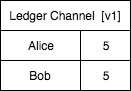
\includegraphics[scale=0.5]{turbo_start} % TODO: tikz
\end{center}

Alice and Bob proceed by creating a new channel $\rchi_C$ for the chess game with the appropriate starting state.
They then update $\rchi_L$ to allocate funds to these games.

\begin{center}
  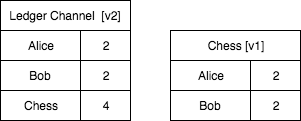
\includegraphics[scale=0.5]{turbo_open} %TODO: tikz
\end{center}

Once the funds are allocated, they are free to play the game of chess.
Updates to the chess channel are independent from updates to $\rchi_L$ and to
any other sub-channels that are potentially funded by it. 
Alice wins the chess game, so the final state in the chess channel allocates all the
funds to her.

\begin{center}
  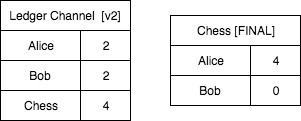
\includegraphics[scale=0.5]{turbo_close} %TODO: tikz
\end{center}

To close the chess channel off-chain, Alice and Bob update the state of the ledger channel to absorb the outcome of the game.

\begin{center}
  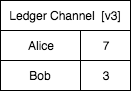
\includegraphics[scale=0.5]{turbo_finish} %TODO: tikz
\end{center}

In the rest of this section we will present the protocol that makes the above interaction
possible.

\subsection{Turbo Outcomes and Operations}

Turbo protocol specifies the interpretation of channel outcomes and the operations that
manipulate them once they are on-chain.
The process of registering the outcome with the chain is not specified, but could be accomplished
using the ForceMove protocol.

Outcomes in Turbo take the form of an ordered list of address-value pairs.
To write outcomes we will use the notation $\{a_1{:}v_1, \dots, a_n{:}v_n \}$, where the $a_i$
represent addresses and the $v_i$ represent values.
The key idea behind Turbo is that the addresses in the outcomes are not limited to being
participant addresses but that they can also be addresses of other \textit{channels}.

The ordering in the outcome is significant and is used to determine a priority order for payouts,
which becomes important if channel does not hold enough funds to cover the entire outcome.

The naive algorithm for distributing the funds is to work along the outcome from the front,
paying funds out to the corresponding address until no funds are remaining.
In practice, we avoid introducing a dependency on the order of the payouts by using
the \textbf{overlap} function $\texttt{overlap}(p, \omega, x)$, which returns the payout owed
to $p$ from outcome $\omega$ when the channel is funded with $x$.
If we have $\adj{\beta_\rchi(\omega)}$ and $\texttt{overlap}(p, \omega, x) = y$, we say that $\rchi$ \textbf{allocates} $y$ to $p$ \textbf{within} $x$.
A python implementation of $\texttt{overlap}$ is given in the appendix.

\begin{figure}[ht]
  \centering
  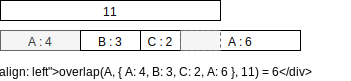
\includegraphics[scale=0.7]{overlap} % TODO: tikz
  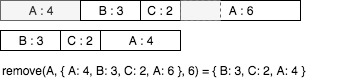
\includegraphics[scale=0.7]{remove} % TODO: tikz
  \caption{Overlap and remove}
\end{figure}

Once an outcome, $\omega$, has paid out a total, $x$, to an address, $A$, we will \textbf{remove} the total to create a new outcome $\omega' = \texttt{remove}(A, \omega, x)$.
The remove operation works through the outcome from the start, reducing the totals for $A$ until $x$ coins have been removed.
A python implementation of $\texttt{remove}$ is given in the appendix.

Armed with overlap and remove, we can now define the only on-chain operation added by Turbo.
The \textbf{transfer} operation, $T_{A,B}(x)$, is an instruction to transfer $x$ coins
currently held by $A$ to $B$, according to the outcome of $A$.

The operation can be described as follows:
if channel $A$ holds at least $a \geq x$ coins
and the outcome, $\beta_A(\omega)$, of $A$ allocates $x$ to $B$ within $a$,
then decrease the total held by $A$ by $x$ coins,
increase the total held by $B$ by $x$ coins
and replace the outcome with $\beta_A(\omega')$, where $\omega' = \texttt{remove}(B, \omega, x)$.
Otherwise, do nothing.
We provide a python implementation of transfer in the appendix.
By way of an example:
\begin{align*}
T_{A,B}(3) \adj{\alpha_A(10)\beta_A(B: 3, C: 7)} = \adj{\alpha_A(7)\alpha_B(3)\beta_A(C: 7)}
\end{align*}

Combined with the deposit and withdrawal operations, the transfer operation gives us everything we need to create a system that supports ledger channels.

\subsection{Value Equivalence in Turbo}

In section \ref{section:value-of-a-state} we defined the value of a system state, $\nu_p(\Sigma)$, to be the to be the largest $x$ such that $p$ has an unbeatable strategy to extract $x$ coins from the adjudicator.
We then split this into two parts: the unbeatable strategy for registering an outcome with the adjudicator and the unbeatable strategy for calling on-chain operations to move the coins into $p$'s address.
We looked a lot at the former part, which gave us the concept of a finalizable state,
but have not yet covered the second part.
In this section, we will look at what it takes to have an unbeatable strategy for moving funds from one address to another in Turbo.

For Turbo it turns out that the rule is very simple: if $p$ has any strategy for withdrawing $x$ coins from the adjudicator, it is an unbeatable strategy.

The following observation about the transfer operation is the key portion of the proof:
if I have the operation $T_{A, B}(x)$, that causes a change to the on-chain state,
then we must have some outcome $\adj{\beta_A(\omega)}$, which means that $A$ is a channel address and therefore withdrawals from $A$ are impossible.
Therefore the only operations that can reduce the total held in $A$ are transfers of the form $T_{A, \rchi}(x)$ for addresses $\rchi$ that appear in $\omega$.
Due to the definition of the transfer operation, all operations of this form commute.
So no transfer operation inserted in front of $T_{A, \rchi}(x)$ can change its effect on the state.

\subsection{Ledger channels}

While this generalization allows for a variety of relationships between different channels,
we will focus here on a setup where a single parent channel funds one or more sub-channels
\footnote{Note that we allow the case where the sub-channels are themselves ledger channels.}.
Following the Perun paper, we will refer to this parent channel as a \textbf{ledger channel}.

All ledger channels in the following sections run the consensus game, so that we can use the value preserving consensus transition result.

\subsubsection{Opening a sub-channel}

In this section, we give the details of the sub-channel opening process that we touched on at the beginning of the Turbo chapter.
We assume we start in a position where we have a ledger channel $L$ between $A$ and $B$, which contains enough to fund a sub-channel, $\rchi$.
This sub-channel runs an arbitrary ForceMove application and starts the process at the funding point, giving the universally finalizable below.
We progress through the following system states:
\begin{align*}
  S_1 &= \adj{\alpha_L(a+b)} &&\enf{\beta_L(A: a, B: b)}_{A, B} & \\
  S_2 &= \adj{\alpha_L(a+b)} &&\enf{\beta_L(A: a, B: b)}_{A, B}&\enf{\beta_\rchi(A: a', B: b')}_{A, B} \\
  S_3 &= \adj{\alpha_L(a+b)} &&\enf{\beta_L(A: a-a', B: b-b', \rchi: x)}_{A, B}&\enf{\beta_\rchi(A: a', B: b')}_{A, B}
\end{align*}
where $x = a' + b'$.
For all of these states, we have $\nu_A(S_i) = a$ and $\nu_B(S_i) = b$.
As each system state only differs in the state of one channel, we can apply the VPCT result, to see that we can move between the system states whilst keeping the system value constant for both $A$ and $B$.
At the end of this process, the funding of the sub-channel is complete and the players can proceed with the non-value preserving interaction within it.

\subsubsection{Closing a sub-channel}

Closing a sub-channel is very similar to opening a sub-channel, involving the same states in the reverse order.
In this instance, the universally finalizable state in the sub-channel, $\rchi$, is
taken to come from a conclusion proof.
\begin{align*}
S_1 &= \adj{\alpha_L(x)} &&\enf{\beta_L(A: a, B: b, \rchi: a' + b')}_{A, B}&\enf{\beta_\rchi(A: a', B: b')}_{A, B}\\
S_2 &= \adj{\alpha_L(x)} &&\enf{\beta_L(A: a + a', B: b + b')}_{A, B}&\enf{\beta_\rchi(A: a', B: b')}_{A, B} \\
S_3 &= \adj{\alpha_L(x)} &&\enf{\beta_L(A: a + a', B: b + b')}_{A, B} & 
\end{align*}
where $x = a + a' + b + b'$.
The analysis here is exactly the same as in the opening case, where $\nu_A(S_i) = a + a'$ and $\nu_B(S_i) = b + b'$.
We then apply the VPCT result to argue that we can transition between these states without changing the value for either player.

\subsubsection{Topping up a ledger channel}

Sometimes it is useful for one participant to be able to increase their total in a ledger channel without disturbing any sub-channels operating in it.
In the scenario below, $A$ and $B$ have a ledger channel, $L$, supporting a sub-channel, $\rchi$, whose state is not shown.
Participant $A$ wants to increase their balance in the channel by an amount $a'$, through an on-chain deposit.
The operation proceeds as follows:
\begin{align*}
S_1 &= \adj{\alpha_L(x)} &&\enf{\beta(A: a, B: b, \rchi: c)}_{A, B} \\
S_2 &= \adj{\alpha_L(x)} &&\enf{\beta(B: b, \rchi: c, A: a + a')}_{A, B} \\
S_3 &= D_L(a')\adj{\alpha_L(x)} &&\enf{\beta(B: b, \rchi: c, A: a + a')}_{A, B} \\
S_4 &= \adj{\alpha_L(x + a')} &&\enf{\beta(B: b, \rchi: c, A: a + a')}_{A, B}
\end{align*}
Here we have $\nu_A(S_1) = \nu_A(S_2) = a + c_A$, $\nu_A(S_3) = \nu_A(S_4) = a + a' + c_A$ and the value to $B$ stays constant at $b + c_B$ throughout, where $c_A$ and $c_B$ is the value attributable to $A$ and $B$, respectively, from the $\rchi$ sub-channel.
The operation starts by moving $A$'s entry to the end of the list.
It is then safe to increase the total to $a + a'$, using the priority order payout property and the fact that the channel is underfunded, to see that this has not changed the value to $A$.
In the next line, $A$ deposits $a'$, which causes the value to $A$ to increase by the same amount, as should happen.
At this point the channel is fully funded and the participants are free to reorder the entries of the outcome as they please.

\subsubsection{Partial checkout from a ledger channel}

A partial checkout is the opposite case to a top up: here $A$ wants to withdraw $a'$ coins from the ledger channel, without disturbing any sub-channels.
The approach here is different to topping up.
The general idea is to replace the ledger channel, $L$, with an equivalent ledger channel, $L'$, with $A$'s balance reduced and then switch the funding across.
For simplicity, we assume that we start with $\adj{\alpha_A(0)}$, so $A$ has no funds held on-chain at the beginning.
\begin{align*}
S_1 &= \adj{\alpha_L(x)} \quad \enf{\beta_L(B: b, A: a, \rchi: c)}_{A, B}  \\
S_2 &= \adj{\alpha_L(x)} \quad \enf{\beta_L(B: b, A: a, \rchi: c)}_{A, B} \quad \enf{\beta_{L'}(B: b, A: a - a', \rchi: c)}_{A, B}\\
S_3 &= \adj{\alpha_L(x)} \quad \enf{\beta_L(L': x-a', A: a')}_{A, B} \quad \enf{\beta_{L'}(B: b, A: a - a', \rchi: c)}_{A, B}\\
S_4 &= \adj{\alpha_L(x)\beta_L(L': x-a, A: a')} \quad \enf{\beta_{L'}(B: b, A: a - a', \rchi: c)}_{A, B}\\
S_5 &= \adj{\alpha_{L'}(x-a')\alpha_A(a')} \quad \enf{\beta_{L'}(B: b, A: a - a', \rchi: c)}_{A, B}
\end{align*}
All these states have the same value for $A$ and $B$.
The first two transitions rely on the VPCT result.
The move from $S_3$ to $S_4$ involves registering the outcome of $L$ on-chain.
It is assumed here that the participants create a conclusion proof, so that they can
skip the timeout.
The final transition involves applying the transfer operations $T_{L, L'}(x-a')$ and $T_{L, A}(a')$.

\section{Nitro Protocol}

Nitro Protocol is an extension to Turbo that introduces a new type of outcome and the on-chain operations to support it. 
We will show how this extension enables a channel between two participants to be supported through a third party.
Following the terminology in the Perun paper, we will refer to these channels as \textbf{virtual channels}.

As an example, suppose that Alice wants to open an $\{A:5, B:5\}$ chess game with Bob, but they do not share an existing ledger channel.
Alice does, however, have an $\{A:5, C:5\}$ ledger channel open with Carol and Bob and Carol have a $\{B:5, C:5\}$ ledger channel open too.

Nitro Protocol allows Alice and Bob to open their chess game, using their existing ledger channels with Carol, without the need for any on-chain transactions.
Suppose that Alice wins all of the funds in the channel, so that the final outcome is $\{A: 10, B: 0\}$.
Then Nitro allows Alice and Bob to close their chess game off-chain too, rebalancing through Carol, so that the final state of the ledger channels is $\{A: 10, C: 0\}$ and $\{B: 0, C: 10\}$.

In this interaction, Carol contributed 10 of her coins at the beginning, which had to remain locked while Alice and Bob were playing.
She got those 10 coins back but they were distributed differently between the her ledger channels.
By locking up her coins for a period of time, she enabled Alice and Bob to play chess entirely off-chain.

In this section, we will introduce the new outcomes and operations, along with the network construction to make interactions like the above possible.

\subsection{Nitro Outcomes and Operations}

Nitro extends Turbo by adding a new type of channel whose outcomes are interpreted differently.
We refer to these new channels as \textbf{guarantor} channels.
In all ways apart from the interpretation of the outcomes, guarantor channels behave exactly like regular channels: they follow the ForceMove update rules and are finalized on-chain in the same way, and they can run ForceMove applications, like the consensus game.

The outcome of a guarantor channel specifies certain parts of another channel's outcome to guarantee.
We will use the notation $\gamma_{A, B}(\omega)$ to represent the outcome, $\omega$, of channel $A$, which is acting as a guarantor for $B$.

Along with the new type of channel, Nitro adds one operation: the \textbf{claim} operation, $G_{A, B, C}(x)$, which is used to claim on the guarantee of $A$ on $B$'s payout to $C$.

Before proceeding with the definitions, we are going to start with some examples to give an idea of how these new additions interact:

\begin{example}
  This example shows the simplest case of claiming on a guarantee:
  \begin{align*}
    G_{A, B, C}(5)\adj{\alpha_A(5)\gamma_{A, B}(C: 5)\beta_B(C:5)} = \adj{\alpha_C(5)}
  \end{align*}
  Guarantor channel $A$ holds 5 and guarantees 5 for $B$s allocation to $C$, within 5.
  $B$ allocates 5 to $C$, so the claim operation is successful, paying 5 from $A$ to $C$ through the outcome of $B$.
\end{example}

\begin{example}
  The next example shows a slightly more complicated case:
  \begin{align*}
    G_{A, B, C}(2)\adj{\alpha_A(3)\gamma_{A, B}(C: 2)\beta_B(C: 3)} = \adj{\alpha_C(2)\alpha_A(1)\beta_B(C:1)}
  \end{align*}
  Here 2 is transferred from $A$ to $C$ through $B$, but this does not completely eliminate $B$'s payout to $C$.
\end{example}

\begin{example}
  The guarantee only goes through if the balances in $\alpha$, $\gamma$ and $\beta$ are all large enough.
  \begin{align*}
    G_{A, B, C}(3)\adj{\alpha_A(3)\gamma_{A, B}(C: 2)\beta_B(C: 3)} = \adj{\alpha_A(3)\gamma_{A, B}(C: 2)\beta_B(C: 3)}
  \end{align*}
  The operation has no effect, as the balance in the guarantee is not high enough.
\end{example}

\begin{example}
  The guarantee can be used to modify the order of payouts:
  \begin{multline*}
    G_{A, B, C}(2)\adj{\alpha_A(2)\gamma_{A, B}(C: 2, D: 1)\beta_B(D: 1, C: 2)} =\\ \adj{\alpha_C(2)\gamma_{A, B}(D: 1)\beta_B(D: 1)}
  \end{multline*}
  Note that in this case, the payout to $C$ went through because it appeared first in the guarantee outcome, even though it was lower priority in $B$'s outcome.
\end{example}

\begin{example}
  Multiple guarantees can also be used to cover the outcome of a single channel:
  \begin{multline*}
    G_{A', B, D}(2)G_{A, B, C}(2)\\\adj{\alpha_A(2)\alpha_{A'}(2)\gamma_{A, B}(C: 2, D: 2)\gamma_{A', B}(C: 2, D: 2)\beta_B(C: 2, D: 2)}\\ = \adj{\alpha_C(2)\alpha_D(2)}
  \end{multline*}
  In this example, we managed to set up a situation where it did not matter which of $A$ and $A'$ went to $C$ and which went to $D$ but $C$ would always receive their funds first.
  This trick will be used in the virtual channel construction.
\end{example}


In order to specify the claim operation, it will be useful to introduce a utility operation first: the \textbf{cap} operation.
By capping outcome $\omega_1$ by $\omega_2$ you ensure that $\omega_1$ will never pay out more to any address $A$ than $\omega_2$ would.
The python code for the cap operation is given in the appendix (\ref{appendix:cap}), so here we will settle for a few examples:
\begin{align*}
  \texttt{cap}(\{A: 10\}, \{A:4\}) &= \{A: 4 \} \\
  \texttt{cap}(\{A: 10\}, \{A:4, B: 2, A: 4\}) &= \{A: 8 \} \\
  \texttt{cap}(\{A: 2, B: 3, A: 3, D: 2\}, \{A: 1, B: 2, A: 2\}) &= \{A: 2, B: 2, A:1\}
\end{align*}

We will use the cap operation to define the \textbf{claim} operation, $T_{A,B,C}(x)$, as follows: if $A$ holds $a$, and the outcome of $A$ capped by the outcome of $B$ allocates $x$ to $C$ within $y$, then decrease the amount held by $A$ by $x$, increase the amount held by $C$ by $x$, remove $x$ from $A$'s allocation to $C$ and also remove $x$ from $B$'s allocation to $C$. A python implementation of the claim operation can be found in \ref{appendix:claim}.

\subsection{Value Calculations}

\begin{multline*}
  T_{B, D}(5)G_{A, B, C}(5)\adj{\alpha_A(5)\alpha_B(5)\gamma_{A, B}(C: 5)\beta_B(C: 5, D: 5)}\\= \adj{\alpha_C(5)\alpha_D(5)}
\end{multline*}

\begin{multline*}
  T_{B, C}(5)\adj{\alpha_A(5)\alpha_B(5)\gamma_{A, B}(C: 5)\beta_B(C: 5, D: 5)} \\= \adj{\alpha_C(5)\alpha_A(5)\gamma_{A, B}(C: 5)\beta_B(D: 5)}
\end{multline*}

\subsection{Virtual Channels}

- outline how we can use guarantee channels to create virtual channels
- the construction we will use is as follows

\begin{figure}[h]\centering
  \begin{tikzpicture}[x = 2cm, y=1cm]
    \node (expanded0) at (0, 0) { \begin{tikzpicture}[x=2cm, y=1cm, framed, background rectangle/.style={draw=black,dashed, rounded corners}] 
  % Specification of nodes (position, etc.)
  \node (a0) at (0,0) { $\adj{\holds{L}{x}{}, \holds{L'}{x}{}}$ };
  \node (b0) at (-1,-1) { $\finalizable{L}{\alloc{A: a, I: b}}{A, I}$ };
  \node (b1) at (1,-1) { $\finalizable{L'}{\alloc{I:a, B:b}}{B, I}$ };
  \node (g0) at (-1,-2) { $\finalizable{G}{\guar{J}{\rchi, A, I}}{A, I}$ };
  \node (g1) at (1,-2) { $\finalizable{G'}{\guar{J}{\rchi, B, I}}{B, I}$ };
  \node (j) at (0,-3) { $\finalizable{J}{\alloc{A: a, B: b, I: x}}{A, B, I}$ };
  \node (c) at (0,-4) { $\finalizable{\rchi}{\alloc{A:a, B: b}}{A, B}$ };

  \begin{scope}[-]
    \tikzstyle{every node}=[draw=none,below]
    \draw (a0) to (b0);
    \draw (a0) to (b1);
    \draw (g0) to (j);
    \draw (g1) to (j);
  \end{scope}

\end{tikzpicture}
 };
    \node[scale=0.4, rectangle, draw, dashed, rounded corners] (state0) at (3, 1.5) { 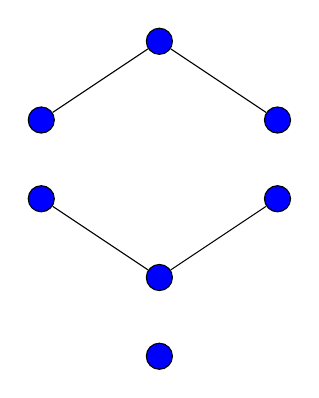
\begin{tikzpicture}[x=1.5cm,y=1cm,every node/.style={draw,solid,shape=circle,fill=blue}]

  % Specification of nodes (position, etc.)
  \node (a0) at (0,0) {};
  \node (b0) at (-1,-1) {};
  \node (b1) at (1,-1) {};
  \node (g0) at (-1,-2) {};
  \node (g1) at (1,-2) {};
  \node (j) at (0,-3) {};
  \node (c) at (0,-4) {};

  \begin{scope}[-]
    \tikzstyle{every node}=[draw,below]
    \draw[solid] (a0) to (b0);
    \draw[solid] (a0) to (b1);
    \draw[solid] (g0) to (j);
    \draw[solid] (g1) to (j);
  \end{scope}

\end{tikzpicture}
 };
    \node[scale=0.4] (state1a) at (4, 1.5) { 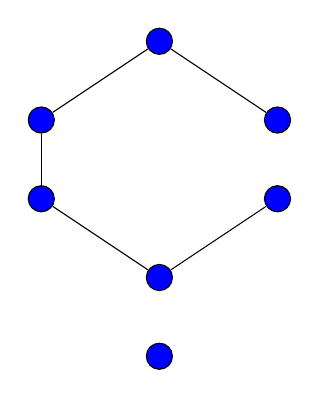
\begin{tikzpicture}[x=1.5cm,y=1cm,every node/.style={draw,shape=circle,fill=blue}]

  % Specification of nodes (position, etc.)
  \node (a0) at (0,0) {};
  \node (b0) at (-1,-1) {};
  \node (b1) at (1,-1) {};
  \node (g0) at (-1,-2) {};
  \node (g1) at (1,-2) {};
  \node (j) at (0,-3) {};
  \node (c) at (0,-4) {};

  \begin{scope}[-]
    \tikzstyle{every node}=[draw=none,below]
    \draw (a0) to (b0);
    \draw (a0) to (b1);
    \draw (b0) to (g0);
    \draw (g0) to (j);
    \draw (g1) to (j);
  \end{scope}

\end{tikzpicture}
 };
    \node[scale=0.4] (state1b) at (3, -1) { 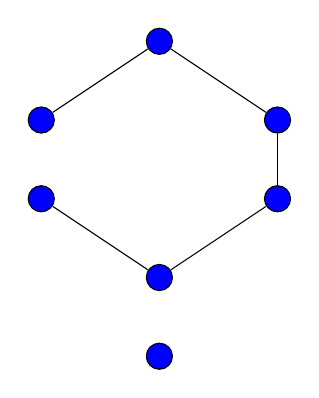
\begin{tikzpicture}[x=1.5cm,y=1cm,every node/.style={draw,shape=circle,fill=blue}]

  % Specification of nodes (position, etc.)
  \node (a0) at (0,0) {};
  \node (b0) at (-1,-1) {};
  \node (b1) at (1,-1) {};
  \node (g0) at (-1,-2) {};
  \node (g1) at (1,-2) {};
  \node (j) at (0,-3) {};
  \node (c) at (0,-4) {};

  \begin{scope}[-]
    \tikzstyle{every node}=[draw=none,below]
    \draw (a0) to (b0);
    \draw (a0) to (b1);
    \draw (b1) to (g1);
    \draw (g0) to (j);
    \draw (g1) to (j);
  \end{scope}

\end{tikzpicture}
 };
    \node[scale=0.4] (state2) at (4, -1) { 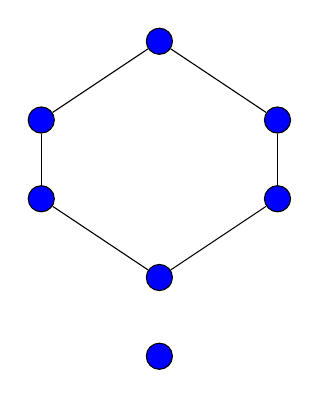
\begin{tikzpicture}[x=1.5cm,y=1cm,every node/.style={draw,shape=circle,fill=blue}]

  % Specification of nodes (position, etc.)
  \node (a0) at (0,0) {};
  \node (b0) at (-1,-1) {};
  \node (b1) at (1,-1) {};
  \node (g0) at (-1,-2) {};
  \node (g1) at (1,-2) {};
  \node (j) at (0,-3) {};
  \node (c) at (0,-4) {};

  \begin{scope}[-]
    \tikzstyle{every node}=[draw=none,below]
    \draw (a0) to (b0);
    \draw (a0) to (b1);
    \draw (b0) to (g0);
    \draw (b1) to (g1);
    \draw (g0) to (j);
    \draw (g1) to (j);
  \end{scope}

\end{tikzpicture}
 };
    \node[scale=0.4, rectangle, draw, dashed, rounded corners] (state3) at (4, -3.5) { 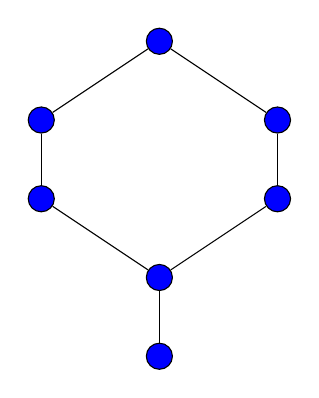
\begin{tikzpicture}[x=1.5cm,y=1cm,every node/.style={draw,solid,shape=circle,fill=blue}]

  % Specification of nodes (position, etc.)
  \node (a0) at (0,0) {};
  \node (b0) at (-1,-1) {};
  \node (b1) at (1,-1) {};
  \node (g0) at (-1,-2) {};
  \node (g1) at (1,-2) {};
  \node (j) at (0,-3) {};
  \node (c) at (0,-4) {};

  \begin{scope}[-]
    \tikzstyle{every node}=[draw=none,below]
    \draw[solid] (a0) to (b0);
    \draw[solid] (a0) to (b1);
    \draw[solid] (b0) to (g0);
    \draw[solid] (b1) to (g1);
    \draw[solid] (g0) to (j);
    \draw[solid] (g1) to (j);
    \draw[solid] (j) to (c);
  \end{scope}

\end{tikzpicture}
 };
    \node (expanded3) at (1, -6) { 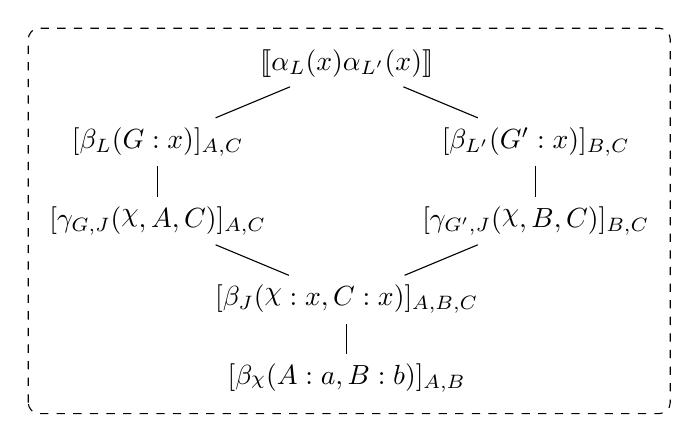
\begin{tikzpicture}[x=2.4cm, y=1cm, framed, background rectangle/.style={draw=black,dashed, rounded corners}] 

  % Specification of nodes (position, etc.)
  \node (a0) at (0,0) { $\adj{\alpha_L(x)\alpha_{L'}(x)}$ };
  \node (b0) at (-1,-1) { $\enf{\beta_L(G: x)}_{A, C}$ };
  \node (b1) at (1,-1) { $\enf{\beta_{L'}(G': x)}_{B, C}$ };
  \node (g0) at (-1,-2) { $\enf{\gamma_{G, J}(\rchi, A, C)}_{A, C}$ };
  \node (g1) at (1,-2) { $\enf{\gamma_{G', J}(\rchi, B, C)}_{B, C}$ };
  \node (j) at (0,-3) { $\enf{\beta_J(\rchi: x, C: x)}_{A,B,C}$ };
  \node (c) at (0,-4) { $\enf{\beta_\rchi(A: a, B: b)}_{A,B}$ };

  \begin{scope}[-]
    \tikzstyle{every node}=[draw=none,below]
    \draw (a0) to (b0);
    \draw (a0) to (b1);
    \draw (b0) to (g0);
    \draw (b1) to (g1);
    \draw (g0) to (j);
    \draw (g1) to (j);
    \draw (j) to (c);
  \end{scope}

\end{tikzpicture}
 };

    \begin{scope}[ultra thick]
      \tikzstyle{every node}=[below]
      \draw[-{Latex[length=3mm,width=4mm]}] (state0) edge (state1a)
                (state0) edge (state1b)
                (state1a) edge (state2)
                (state1b) edge (state2)
                (state2) edge (state3);
    \end{scope}
  \end{tikzpicture}
  \caption{Ledger channels, $x = a + b$}
  \label{fig:modes}
\end{figure} 


- worth thinking about how this works
- offload
- key is the joint A-B-C channel, source of truth for state of channel


\subsubsection{Opening a Virtual Channel}

Want to start in the situation where channels A-C and B-C exist and demonstrate how to
open the virtual channel situation

- first create the subchannel we want to fund
- and the joint channel and guarantee channels to support it
everything here is disconnected
- then we update the ledger channels, one at a time to fund the guarantees
- finally we update the joint channel to fund the virtual channel

\subsubsection{Closing a Virtual Channel}

Opening a channel in reverse
- start with the virtual channel coming to a finalizable outcome e.g. conclude
- then A or B propose an update to j
- once A and B have signed off, it's in C's interest too
- then they can defund the guarantee channels independently


\section{Acknowledgements}

- Andrew Stewart
- James Prestwich
- Chris Buckland
- Magmo team


\section{Appendix}

\subsection{Overview of ForceMove}
\subsection{The Consensus Game}
\subsection{Virtual Channels on Turbo}
\subsection{Payouts to Non-Participants}
\subsection{Possible Extensions}

\subsection{On-chain Operations Code}
\subsubsection{Overlap}
\begin{minipage}{\linewidth} % minipage to avoid page breaks
  \lstinputlisting[language=Python]{code/overlap.py}
\end{minipage}

\subsubsection{Remove}
\begin{minipage}{\linewidth} % minipage to avoid page breaks
  \lstinputlisting[language=Python]{code/remove.py}
\end{minipage}

\subsubsection{Transfer}
\begin{minipage}{\linewidth} % minipage to avoid page breaks
  \lstinputlisting[language=Python]{code/transfer.py}
\end{minipage}

\subsubsection{Cap}\label{appendix:cap}
\begin{minipage}{\linewidth} % minipage to avoid page breaks
  \lstinputlisting[language=Python]{code/cap.py}
\end{minipage}

\subsubsection{Claim}\label{appendix:claim}
\begin{minipage}{\linewidth} % minipage to avoid page breaks
  \lstinputlisting[language=Python]{code/claim.py}
\end{minipage}

\end{document}
